\title{Assinatura geomorfométrica: potencial para estudos pedométricos}
\author{por Vinicius Vasconcelos}
\maketitle
\begin{wrapfigure}{l}{0.15\textwidth}
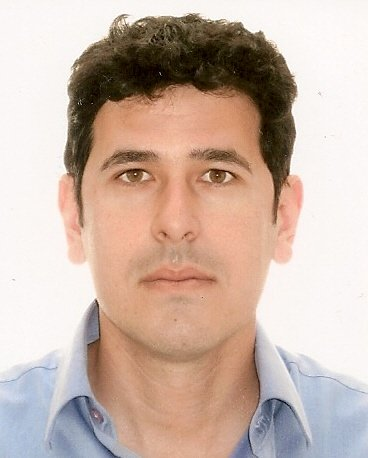
\includegraphics[width=0.15\textwidth]{figuras/foto-vini.jpg}
\end{wrapfigure}
Muitos estudos têm sido realizados para obter uma descrição detalhada das formas de terreno com o propósito de compreender a evolução da paisagem. Nesta perspectiva, consolida-se o campo da ciência denominada de \emph{(Geo)morfometria} que analisa a superfície topográfica de forma quantitativa. Esta disciplina também é conhecida como \emph{análise de terreno} ou \emph{modelagem digital de terreno} \citep{LaneEtAl1998, Pike:2000}.\\
Um dos pressupostos levantados pela Geomorfometria é a obtenção das feições do relevo de maneira automática ou semi-automática.  É importante citar alguns trabalhos dentro dessa perspectiva. Eu começaria por \cite{Wood:1996}, uma tese de doutorado disponível no endereço \url{http://www.soi.city.ac.uk/~jwo/phd/}. O autor obteve seis feições morfométrica conhecidas como \emph{peak}, \emph{pass}, \emph{channel}, \emph{pit}, \emph{plane} e \emph{ridge} a partir de curvaturas, vertical, longitudinal, transversal, mínima e máxima.  O método considera uma combinação específica dos pares de curvaturas Longitudinal/Transversal e Mínima/Máxima a depender da declividade da região a ser classificada. Assim, as curvaturas Longitudinal/Transversal são apenas utilizadas quando o relevo apresenta uma declividade mais acentuada. Consequentemente, as curvaturas e Mínima e Máxima são utilizadas em áreas de relevo mais suave. Desta forma, a combinação das curvaturas apresenta uma relação excludente de acordo com o relevo que 
será modelado.\\
A observação das curvaturas como parâmetro da análise na identificação do tipo de solo é muito antiga.  \cite{Aandahl:1948} foi o primeiro a reconhecer a influência das curvaturas de plano e de perfil na formação e distribuição dos solos. \cite{Troeh:1964} desenvolveu o primeiro método quantitativo para estimar curvaturas horizontais e verticais e relacioná-los com as propriedades dos solos. \cite{Pennock:1987} em seguida definiu, por meio das curvaturas verticais e horizontais, uma combinação das primeiras Formas de Terreno (FT) ou \emph{landforms} para estudo de solos.\\
O trabalho que está em desenvolvimento no Laboratório de Sistema de Informações Espaciais (LSIE) do Departamento de Geografia da Universidade de Brasília - UnB, tem como perspectiva compreender melhor a evolução do relevo a partir dos atributos pedológicos a partir técnicas de classificação de Formas de Terreno. O nosso trabalho mais recente é na elaboração de uma curva que possa explicar as variações da intensidade do relevo.\\
Nesse estudo utilizamos dados de curvatura: Vertical, Longitudinal, Transversal, Mínimo, Máximo e Horizontal organizados em uma só imagem com bandas de curvatura com consequente formação de uma  assinatura geomorfométrica \citep{Vasconcelos:2012}. Esta assinatura consiste na formulação de uma curva das medidas topográficas capaz de distinguir as diferentes paisagens. Assim, cada célula da grade (unidade de terreno) é descrita por uma curva dos atributos de terreno que pode ser comparada com curvas específicas de formas de relevo (assinaturas). Esta abordagem conduz ao emprego de técnicas de reconhecimento de padrões a partir de métodos estatísticos multivariados comumente empregados no processamento digital de imagens de sensoriamento remoto \citep{BrownEtAl:1998}.\\
Primeiramente é utilizado o método Menor Fração de Ruído (MFR). Esse método funciona como uma Análise de Principal Componente, determina a dimensionalidade inerente dos dados de imagem, para separar o ruído nos dados, e reduzir os requisitos de cálculo para um processamento subsequente \citep{BoardmanEtAl:1994}. Em uma imagem composta por curvaturas, o MFR vai selecionar as informações que mais se repetem na imagem. Em seguida, utiliza-se outro método para por fim identificar as assinaturas geomorfométricas: Indice de Pureza do Pixel. Esse processamento foi desenhado para localizar os mais extremos (valor único ou diferente ou "puro"), pixels \citep{BoardmanEtAl:1995}. Os pixels mais puros tipicamente correspondem a um membro final, ou seja, uma curva padrão de forma de terreno.\\
O método de assinatura geomorfométrica reconhece não só o padrão de uma Forma de Terreno, mas também a sua intensidade, permitindo identificar e classificar inúmeras formas. Nesse sentido, esse procedimento pode auxiliar na escolha de áreas de referência para estudos pedológicos assim como na relação solo-paisagem.
\begin{footnotesize}
\begin{thebibliography}{99}
\bibitem[Boardman et~al. (1994) Boardman, Kruse]{BoardmanEtAl:1994}
J.W. Boardman, F.A. Kruse (1994)
\newblock Automated  spectral analysis a geological example using AVIRIS data, North Grapevine, Mountains, Nevada.
\newblock {\em Proceedings of the Tenth Thematic Conference on Geological Remote Sensing, San Antonio} pp.407-418.
\bibitem[Boardman et~al. (1995) Boardman, Kruse, Green]{BoardmanEtAl:1995}
J.W. Boardman, F.A. Kruse, R.O. Green (1995)
\newblock Mapping target signatures via partial unmixing of AVIRIS data
\newblock {\em Annual JPL Airborne Geosciences Workshop, Pasadena} pp.23-26.
\bibitem[Brown et~al. (1998) Brown, Lusch, Duda]{BrownEtAl:1998}
D.G. Brown, D.P. Lusch, K.A. Duda (1998)
\newblock Supervised classification of glaciated landscape types using digital elevation data.
\newblock {\em Geomorphology} 21: 233-250.
\bibitem[Lane et~al. (1998) Lane, Richards, Chandler]{LaneEtAl1998}
S.N. Lane, K.S. Richards, J.H. Chandler (1998)
\newblock Landform Monitoring, Modelling and Analysis.
\newblock {\em Wiley} 466 pp.
\bibitem[Jo Wood (1996)]{Wood:1996}
J. Wood (1996)
\newblock The  Geomorphological  Characterisation of Digital Elevation Models.
\newblock {\em Thesis (PhD in Science Information)} 184p.
\bibitem[Aandahl (1948)]{Aandahl:1948}
A.R. Aandahl (1948)
\newblock The characterization of slope positions and their influence on the total N content of a few virgin soils in Western Iowa.
\newblock {\em Soil Science Society of America Journal} 13: 449–454.
\bibitem[Troeh (1964)]{Troeh:1964}
F.R. Troeh (1964)
\newblock Landform parameters correlated to soil drainage.
\newblock {\em Soil Science Society of America Journal} 28: 808–812.
\bibitem[Pennock et~al. (1987) Pennock, Zebarth, De Jong]{Pennock:1987}
D.J. Pennock, B.J. Zebarth, E. De Jong (1987)
\newblock Landform  Classification  and  Soil Distribution in Hummocky Terrain, Saskatchewan, Canada.
\newblock {\em Geoderma} 40: 297-315.
\bibitem[Pike (2000) Pike]{Pike:2000}
R.J. Pike (2000)
\newblock Geomorphometry — diversity in quantitative surface analysis.
\newblock {\em Progress in Physical Geography} 24: 1-20.
\bibitem[Vasconcelos et~al. (2012) Vasconcelos, Carvalho Junior, Martins, Guimarães, Gomes]{Vasconcelos:2012}
V. Vasconcelos, O.A. Carvalho Junior, E.S. Martins, A.F. Couto Junior, R.F. Guimarães, R.A.T. Gomes (2012)
\newblock Sistema de Classificação Geomorfométrica baseado em uma arquitetura sequencial em duas etapas: Árvore de Decisão e Classificador Espectral, no Parque Nacional da Serra da Canastra.
\newblock {\em Revista Brasileira de Geomorfologia} 13: 171-186.
\end{thebibliography}
\end{footnotesize}
\address{Vinicius Vasconcelos\\
  Universidade de Brasília\\
  \email{vinicius.vascoza@gmail.com}}
%%% Local Variables: 
%%% mode: latex
%%% TeX-master: documento-principal.tex
%%% End: